\documentclass[12pt, a4paper, onecolumn, notitlepage]{article}

\usepackage[utf8]{inputenc}
\usepackage{indentfirst}
\usepackage{graphicx}
\usepackage{caption}
\usepackage{url}
\usepackage{tabularx}
\usepackage{ragged2e}
\usepackage{longtable}

\begin{document}
    \section*{Desafio 1 - Método CO-STAR}
    \textbf{Desafio:} Escolha uma região ou município da Amazônia Legal onde o desmatamento aumentou nos últimos dois anos. Utilizando fontes confiáveis (MapBiomas, Imazon, INPE), analise os fatores associados ao aumento e proponha uma solução tecnológica ou educativa apoiada em IA.

    \section[short]{Introdução}
    Neste trabalho, é abordado o aumento do desmatamento no município de Acará, localizado no estado do Pará, na Amazônia Legal. O município de Acará possui 4.300 km² de área e uma população de aproximadamente 50.000 habitantes, segundo o IBGE~\footnote{Dados do IBGE: \url{https://cidades.ibge.gov.br/brasil/pa/acara/panorama.html}}. O Acará possui cerca de 65\% de área florestal incluíndo as áreas de Floresta Alagável, sendo a outra maior porcentagem de áreas relacionadas a agropecuária voltada a pastagem e agricultura como demonstra a Figura~\ref{fig:territorio_acara}.

    \begin{figure}[htbp]
        \centering
        \caption*{Fonte: MapBiomas}
        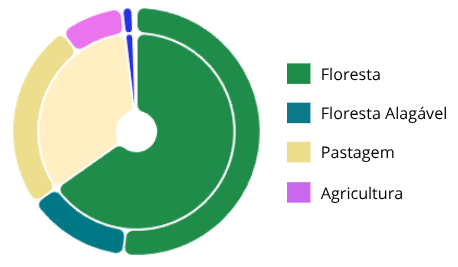
\includegraphics[width=0.6\textwidth]{figures/territorio_acara.png}
        \caption{Território de Acará, Pará, destacando áreas florestais e agropecuárias.}
        \label{fig:territorio_acara}
    \end{figure}
    
    Segundo dados do MapBiomas Alerta, o desmatamento na região no ano de 2024 cresceu cerca de 20\% em relação ao ano de 2023 (Figura~\ref{fig:grafico_desmatamento_2023_2024}).

    \begin{figure}[htbp]
        \centering
        \caption*{Fonte: MapBiomas Alerta}
        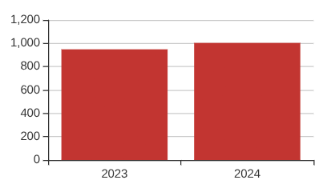
\includegraphics[width=0.6\textwidth]{figures/grafico_desmatamento_2023_2024.png}
        \caption{Gráfico de desmatamento em Acará, Pará, comparando os anos de 2023 e 2024.}
        \label{fig:grafico_desmatamento_2023_2024}
    \end{figure}

    Essa evolução do desmatamento fica ainda mais evidente ao explorar os dados no MapBiomas Alerta, que mostram com mais detalhes os meses com seus devidos índices de desmatamento como é apresentado na Figura~\ref{fig:grafico_desmatamento_meses_2023_2024}.

    \begin{figure}[htbp]
        \centering
        \caption*{Fonte: MapBiomas Alerta}
        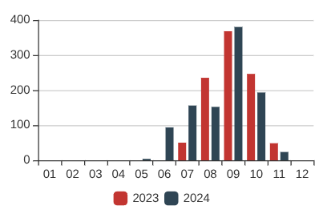
\includegraphics[width=0.6\textwidth]{figures/grafico_desmatamento_meses_2023_2024.png}
        \caption{Gráfico de desmatamento em Acará, Pará, comparando os meses de 2023 e 2024.}
        \label{fig:grafico_desmatamento_meses_2023_2024}
    \end{figure}

    O aumento do desmatamento em Acará pode ser atribuído a diversos fatores interconectados. Primeiramente, a expansão da agricultura e a exploração madeireira ilegal têm exercido pressão significativa sobre os recursos florestais da região. Além disso, a falta de fiscalização efetiva permite que essas atividades ocorram sem o devido controle ambiental. A situação é agravada pela presença de um grande número de indústrias na região, conforme demonstrado pelo ranking do site EMPRESAQUI~\footnote{Ranking das 100 maiores empresas em Acará/PA: \url{https://www.empresaqui.com.br/listas-de-empresas/PA/ACARA}}, que, combinada com a riqueza em recursos naturais locais, cria um cenário propício para a intensificação da degradação ambiental, o mapa de Acará, Pará, apresentado na Figura~\ref{fig:mapa_acara} ilustra a localização geográfica do município e sua proximidade com áreas de desmatamento com maior acentuação no sul do município.

    \begin{figure}[htbp]
        \centering
        \caption*{Fonte: MapBiomas Alerta}
        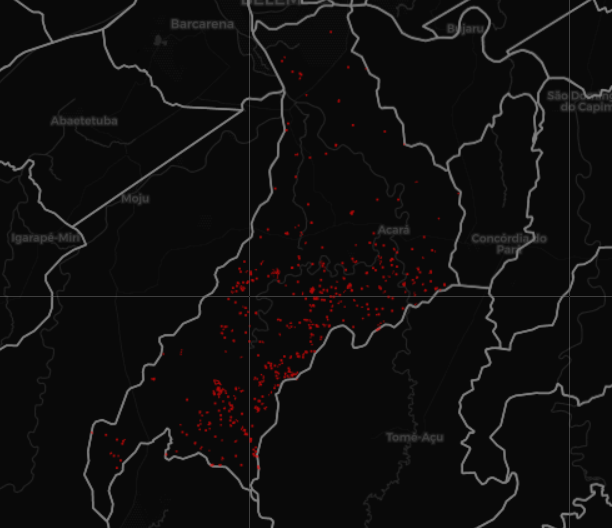
\includegraphics[width=0.8\textwidth]{figures/mapa_acara.png}
        \caption{Mapa de Acará, Pará, destacando áreas de desmatamento.}
        \label{fig:mapa_acara}
    \end{figure}

    Dessa forma, para combater o aumento do desmatamento em Acará e regiões próximas, a Polícia Civil do Pará, por meio da Delegacia de Repressão a Crimes Contra a Flora (DRCCF), deflagrou a operação ``Segredo'' nos municípios de Acará, Tailândia, Moju, Mocajuba e Cametá~\footnote{Noticia da Polícia Civil: \url{https://www.pc.pa.gov.br/noticia/7563}}. A ação, realizada entre 27 e 30 de maio de 2025, teve como objetivo combater crimes de desmatamento ilegal e cumprir requisições ministeriais, utilizando informações da Central de Monitoramento Ambiental que identificou alertas de desmatamento nas regiões. Durante as diligências, foi localizada uma extração clandestina de madeira em Moju, resultando na apreensão de um caminhão carregado com madeiras em tora, duas máquinas (pá carregadeira e trator skid), uma motosserra, aproximadamente 100 toras de madeira derrubadas e duas armas de fogo. Cinco suspeitos foram autuados pelos crimes previstos nos Artigos 50 e 51 da Lei Ambiental 9605/98 e pelo Artigo 12 do Estatuto do Desarmamento, a operação evidencia a gravidade.

    \section{Metodologia Aplicada}
    A metodologia aplicada neste trabalho segue o método CO-STAR, que consiste em:
    \begin{itemize}
        \item \textbf{C}ontextualizar o problema: Analisar o aumento do desmatamento em Acará, Pará, e identificar os fatores associados.
        \item \textbf{O}bservar: Coletar dados de fontes confiáveis como MapBiomas, Imazon e INPE.
        \item \textbf{S}intetizar: Resumir os dados coletados e identificar os principais fatores de desmatamento.
        \item \textbf{T}ransformar: Propor soluções tecnológicas ou educativas baseadas em Inteligência Artificial (IA) para combater o desmatamento.
        \item \textbf{A}plicar: Implementar as soluções propostas e avaliar seu impacto.
        \item \textbf{R}efletir: Analisar os resultados obtidos e propor melhorias para as soluções implementadas.
    \end{itemize}

    O chat utilizado no refinamento do prompt foi o chat GPT-4, e então para gerar a resposta a apartir do prompt refinado, foi utilizado o chat Gemini 2.5 Pro, além disso, foram utilizados os seguintes sites para a coleta de dados em formato pdf:
    \begin{itemize}
        \item MapBiomas Alerta: \url{https://alerta.mapbiomas.org/}
        \item Imazon: \url{https://imazon.org.br/}
        \item INPE: \url{https://www.gov.br/inpe/pt-br}
        \item EMPRESAQUI: \url{https://www.empresaqui.com.br/}
        \item Polícia Civil do Pará: \url{https://www.pc.pa.gov.br/}
        \item IBGE: \url{https://cidades.ibge.gov.br/brasil/pa/acara/panorama.html}
        \item MapBiomas: \url{https://mapbiomas.org/}
        \item G1: \url{https://g1.globo.com/pa/para/noticia/2025/05/30/policia-civil-do-para-deflagra-operacao-segredo-contra-desmatamento-em-acara.ghtml}
    \end{itemize}

    Somadas a essas informações, foi utilizado como base de conhecimento a Introdução elaborada desse documento, com a intenção de filtrar e gerar informações mais precisas sobre o desmatamento em Acará.

    \section{Prompts Utilizados}
    \subsection{Prompt 1}
    Atue como um especialista ambiental com experiência em análise de dados sobre desmatamento na Amazônia Legal. Sua tarefa é analisar todos os documentos e informações disponíveis sobre o desmatamento especificamente no município de Acará, no estado do Pará.

    Realize uma análise aprofundada para identificar os principais fatores que têm contribuído para o aumento do desmatamento na região, considerando aspectos ambientais, socioeconômicos, políticos ou tecnológicos. Em seguida, proponha pelo menos duas soluções baseadas em tecnologias de inteligência artificial, que podem ser de natureza educativa ou técnica (por exemplo, sistemas de monitoramento, plataformas de ensino automatizadas, algoritmos de previsão, etc.).

    Apresente os resultados em formato de tabela, com as colunas:

    Fator

    Descrição

    Consequência

    Possível Solução com IA

    Após a tabela, forneça uma explicação breve e clara dos principais pontos levantados, com uma linguagem acessível ao público geral interessado em temas ambientais.

    Por fim, forneça um resumo final apenas com os insights que propõem soluções tecnológicas ou educativas baseadas em IA, destacando de forma concisa como essas soluções podem ajudar a combater o desmatamento em Acará.

    \section{Resultado dos Prompts}
    \subsection{Prompt 1}

    \subsubsection*{Análise do Desmatamento em Acará (PA) e Soluções com Inteligência Artificial}

    O município de Acará, no estado do Pará, tem enfrentado um aumento preocupante nos índices de desmatamento, impulsionado por uma combinação complexa de fatores. Uma análise aprofundada dos dados e informações disponíveis revela um cenário que exige ações coordenadas e inovadoras para a proteção de suas florestas.

    De acordo com dados do MapBiomas Alerta, o desmatamento em Acará apresentou um crescimento de aproximadamente 20\% em 2024 em comparação com o ano de 2023. Essa tendência se insere no contexto mais amplo do estado do Pará, que liderou o ranking de desmatamento na Amazônia Legal em 2024 pelo nono ano consecutivo, registrando um aumento de 3\% na área desmatada em relação ao ano anterior. Além do corte raso, a degradação florestal, principalmente por queimadas, também é um problema crítico na região, tendo o Pará registrado um aumento de 421\% nessa modalidade de dano ambiental em 2024.

    Operações como a ``Segredo'', deflagrada em maio de 2025 pela Polícia Civil do Pará, buscam combater o desmatamento ilegal em Acará e municípios vizinhos, atuando com base em alertas de desmatamento identificados por centrais de monitoramento. Essas ações policiais têm resultado na apreensão de equipamentos e na autuação de criminosos ambientais, evidenciando a exploração madeireira ilegal como um dos principais vetores.

    A seguir, apresentamos uma tabela que resume os principais fatores de desmatamento em Acará, suas consequências e possíveis soluções utilizando Inteligência Artificial (IA):

    \subsubsection*{Breve Explicação dos Principais Pontos}
    O desmatamento em Acará é um problema multifatorial. A \textbf{expansão da fronteira agropecuária  e a exploração madeireira ilegal}  são vetores diretos da derrubada da floresta, muitas vezes facilitados por \textbf{falhas na fiscalização e em processos de licenciamento ambiental}. A situação é agravada pela \textbf{pressão exercida por grandes projetos de infraestrutura} que, além do impacto direto, geram conflitos com comunidades indígenas e quilombolas que denunciam desmatamento e falta de consulta prévia.

    A \textbf{complexidade das questões fundiárias}, incluindo a grilagem de terras, cria um ambiente de ilegalidade que favorece o desmatamento. Adicionalmente, a \textbf{degradação florestal causada por queimadas}  –- um problema que tem se intensificado em todo o estado do Pará  –- compromete a resiliência da floresta e contribui significativamente para as emissões de carbono. Por fim, a \textbf{carência de alternativas econômicas sustentáveis} para as populações locais mantém a pressão sobre os recursos naturais.

    Ações de comando e controle, como a Operação ``Segredo'', são cruciais, mas a complexidade do problema exige também soluções estruturantes e o uso de novas tecnologias.

    \subsubsection*{Resumo Final: Soluções Tecnológicas e Educativas com Inteligência Artificial}
    Para combater o desmatamento em Acará, propõem-se as seguintes soluções baseadas em Inteligência Artificial:

    \begin{longtable}{@{} | >{\RaggedRight\arraybackslash}p{0.15\textwidth} | >{\RaggedRight\arraybackslash}p{0.25\textwidth} | >{\RaggedRight\arraybackslash}p{0.25\textwidth} | >{\RaggedRight\arraybackslash}p{0.27\textwidth} | @{}}
    % Legenda da tabela
    \hline
    % Cabeçalho da primeira página
    \textbf{Fator} & \textbf{Descrição} & \textbf{Consequência} & \textbf{Possível Solução com IA} \\
    \hline
    \endfirsthead

    % Cabeçalho para as páginas seguintes
    \multicolumn{4}{c}%
    {{\bfseries Tabela \thetable{} -- Continuação da página anterior}} \\
    \hline
    \textbf{Fator} & \textbf{Descrição} & \textbf{Consequência} & \textbf{Possível Solução com IA} \\
    \hline
    \endhead

    % Rodapé para todas as páginas, exceto a última (opcional)
    % \hline
    % \multicolumn{4}{r}{{Continua na próxima página}} \\
    \endfoot

    % Rodapé apenas para a última página (opcional)
    \hline
    \endlastfoot

    % Conteúdo da tabela
    Expansão da Agropecuária &
    Conversão de áreas de floresta para pastagens e agricultura, impulsionada pela demanda por commodities. &
    Perda de biodiversidade, fragmentação de habitats, emissão de gases de efeito estufa (GEE), compactação e erosão do solo. &
    Modelagem Preditiva Agropecuária com IA: Desenvolver algoritmos que prevejam áreas de expansão agrícola de alto risco, auxiliando no planejamento territorial, na fiscalização preventiva e no incentivo a práticas agropecuárias sustentáveis e de baixo carbono em áreas já consolidadas. \\
    \hline

    Exploração Madeireira Ilegal &
    Extração de madeira sem manejo florestal sustentável, sem autorização dos órgãos competentes ou em desacordo com a legislação ambiental. &
    Degradação florestal, esgotamento de espécies de valor econômico, aumento de conflitos e violência, prejuízos à economia formal da madeira. &
    Detecção Avançada de Exploração Ilegal com IA: Utilizar IA para analisar imagens de satélite (ótica e radar) e dados de sensores acústicos para identificar em tempo real atividades de extração seletiva, abertura de ramais e acampamentos madeireiros ilegais, otimizando a resposta dos órgãos fiscalizadores. \\
    \hline

    Falhas na Fiscalização e Licenciamento &
    Capacidade operacional e recursos limitados dos órgãos ambientais para monitorar extensas áreas, coibir atividades ilegais e agilizar processos de licenciamento de forma rigorosa. &
    Sensação de impunidade, perpetuação de atividades ilegais, aumento do desmatamento e da degradação. &
    Otimização da Fiscalização e Análise de Licenças com IA: Implementar sistemas de IA que otimizem rotas de fiscalização baseadas em alertas de desmatamento e predição de risco. Utilizar IA para analisar pedidos de licenciamento ambiental, identificando inconsistências, fraudes ou alto risco ambiental. \\
    \hline

    Pressão de Grandes Projetos de Infraestrutura e Conflitos Socioambientais &
    Implantação de projetos como minerodutos, hidrelétricas e estradas que podem causar desmatamento direto e indireto, além de gerar conflitos com comunidades locais e tradicionais. &
    Desmatamento, fragmentação de ecossistemas, impactos nos recursos hídricos, remoção de comunidades, violação de direitos territoriais. &
    Monitoramento Participativo e Mediação de Conflitos com IA: Criar plataformas baseadas em IA que permitam às comunidades locais reportar impactos de grandes projetos e atividades ilegais. A IA pode auxiliar na análise desses dados e na facilitação do diálogo e mediação de conflitos entre partes. \\
    \hline

    Questões Fundiárias e Grilagem de Terras &
    Incerteza jurídica sobre a posse da terra, processos lentos de regularização fundiária de territórios tradicionais e áreas de conservação, e ocupação ilegal de terras públicas (grilagem). &
    Aumento da especulação imobiliária, desmatamento para demarcação de posse ilegal, conflitos agrários. &
    Agilização da Regularização Fundiária com IA: Empregar ferramentas de IA para acelerar a análise de dados geoespaciais, imagens de satélite históricas e documentos em processos de regularização fundiária, identificando sobreposições, desmatamento ilegal em áreas reivindicadas e indícios de grilagem. \\
    \hline

    Degradação Florestal por Queimadas &
    Uso do fogo para limpeza de áreas desmatadas ou renovação de pastagens que frequentemente se alastram para florestas adjacentes, intensificado por períodos de seca extrema. &
    Perda de biodiversidade, empobrecimento do solo, emissão massiva de GEE, problemas de saúde pública devido à fumaça, alteração do regime hídrico. &
    Sistema Preditivo e de Alerta de Incêndios Florestais com IA: Desenvolver modelos de IA que integrem dados meteorológicos, de umidade da vegetação, focos de calor e histórico de ocorrências para prever áreas de alto risco de incêndios e emitir alertas precoces para brigadas e comunidades. \\
    \hline

    Falta de Alternativas Econômicas Sustentáveis &
    Dependência de comunidades locais de atividades predatórias por ausência de incentivos, conhecimento técnico e acesso a mercados para produtos da sociobiodiversidade e práticas sustentáveis. &
    Pressão contínua sobre os recursos florestais para subsistência ou geração de renda, dificultando a conservação. &
    Plataforma Educacional e de Fomento à Bioeconomia com IA (Proposta 1): Ver resumo abaixo. \\

\end{longtable}


    \begin{enumerate}
        \item \textbf{Sistema Integrado de Monitoramento Avançado e Previsão de Desmatamento com IA (Técnica):} Esta solução consiste no desenvolvimento e implementação de uma plataforma de IA que integre dados de múltiplas fontes (satélites de alta resolução, alertas de desmatamento como os da Central de Monitoramento da Demapa, dados de Cadastro Ambiental Rural, informações sobre cadeias produtivas e rotas de transporte). A IA seria utilizada para:
        \begin{itemize}
            \item \textbf{Detectar em tempo quase real} o desmatamento e a degradação florestal (incluindo extração seletiva e cicatrizes de queimadas) com maior precisão.
            \item \textbf{Prever áreas com alto risco de desmatamento futuro}, analisando padrões de expansão, pressões econômicas e vulnerabilidades socioambientais.
            \item \textbf{Otimizar as ações de fiscalização}, direcionando equipes de forma mais eficiente, gerando alertas automatizados e fornecendo dossiês qualificados para embasar operações de combate a crimes ambientais.
        \end{itemize}

        \item \textbf{Plataforma Educacional Interativa e de Apoio a Alternativas Sustentáveis com IA (Educacional/Técnica):} Esta solução visa engajar e capacitar as comunidades locais, incluindo agricultores familiares, indígenas e quilombolas, através de:
        \begin{itemize}
            \item \textbf{Conteúdo educativo personalizado por IA} sobre a importância da conservação, legislação ambiental, direitos territoriais e os impactos do desmatamento e das queimadas.
            \item \textbf{Módulos de capacitação em práticas sustentáveis}, como sistemas agroflorestais, manejo florestal comunitário, agricultura de baixo carbono e bioeconomia, conectando os usuários a cadeias de valor e mercados justos.
            \item \textbf{Ferramentas de ciência cidadã e monitoramento comunitário}, permitindo que os moradores locais reportem atividades ilegais de forma segura e eficaz, com a IA auxiliando na triagem e encaminhamento das denúncias, fortalecendo o controle social e a governança territorial.
            \item \textbf{Chatbots educativos} para sanar dúvidas sobre regularização ambiental e práticas sustentáveis.
        \end{itemize}
    \end{enumerate}

    Estas soluções de IA, ao combinar o fortalecimento da fiscalização com o empoderamento e a oferta de alternativas para as comunidades locais, podem contribuir significativamente para a redução do desmatamento e para a promoção de um desenvolvimento mais sustentável no município de Acará.
    

    \section{Conclusão}
    A IA generativa Gemini, forneceu informações relevantes sobre o desmatamento em Acará, e propôs soluções robustas com base nas informações pesquisadas e verificadas de forma humana. A análise dos dados coletados revelou a complexidade do problema do desmatamento na região. No entando, sem a intervenção humana para ``checkar'' as informações com precisão, as repostas geradas apesar de seguir qualquer que seja as boas práticas apresentadas em \emph{frameworks}, acabará sendo imprecisa, e por isso é importante que haja uma análise humana para validar as informações geradas por IA, para não propagar desinformação e equívocos principalmente em ambiente academico e cientifico.

    \begin{itemize}
        \item \textbf{Aluno:} Felipe Barbosa
    \end{itemize}
    
\end{document}


